\documentclass[10pt]{article}
\usepackage[margin=0.75in]{geometry}
\usepackage{graphicx}
\usepackage{booktabs}
\usepackage[T1]{fontenc}
\setlength{\parindent}{0pt}
\setlength{\parskip}{6pt}
\begin{document}
\begin{center}
{\Large Source-pinned replay of BINSTD ell89 toy panels}\\[3pt]
2026-10-22 \quad EXP-BINSTD-8bdf86 \quad H-BINSTD-5a212b
\end{center}

This validation replay used the historical code commits recorded in the two
run environments and copied their hash-matched Stage-0 freeze files into
isolated temporary directories. It did not write to any frozen run record.
This is not a new experiment or evidence decision.

\begin{center}
\begin{tabular}{llrrrr}
\toprule
Panel / Stage-1 run & $\ell$ & Tau hits & Open hits & $R_\tau/R_{\rm open}$ & Band \\
\midrule
ell89 / RUN-BINSTD-43abd4 & 8 & 16/40 & 40/40 & 0.4 & 1.25 \\
ell89 / RUN-BINSTD-43abd4 & 9 & 40/40 & 40/40 & 1.0 & 1.25 \\
ell89r1 / RUN-BINSTD-a2a24c & 8 & 20/40 & 40/40 & 0.5 & 1.25 \\
ell89r1 / RUN-BINSTD-a2a24c & 9 & 40/40 & 40/40 & 1.0 & 1.25 \\
\bottomrule
\end{tabular}
\end{center}

\begin{center}
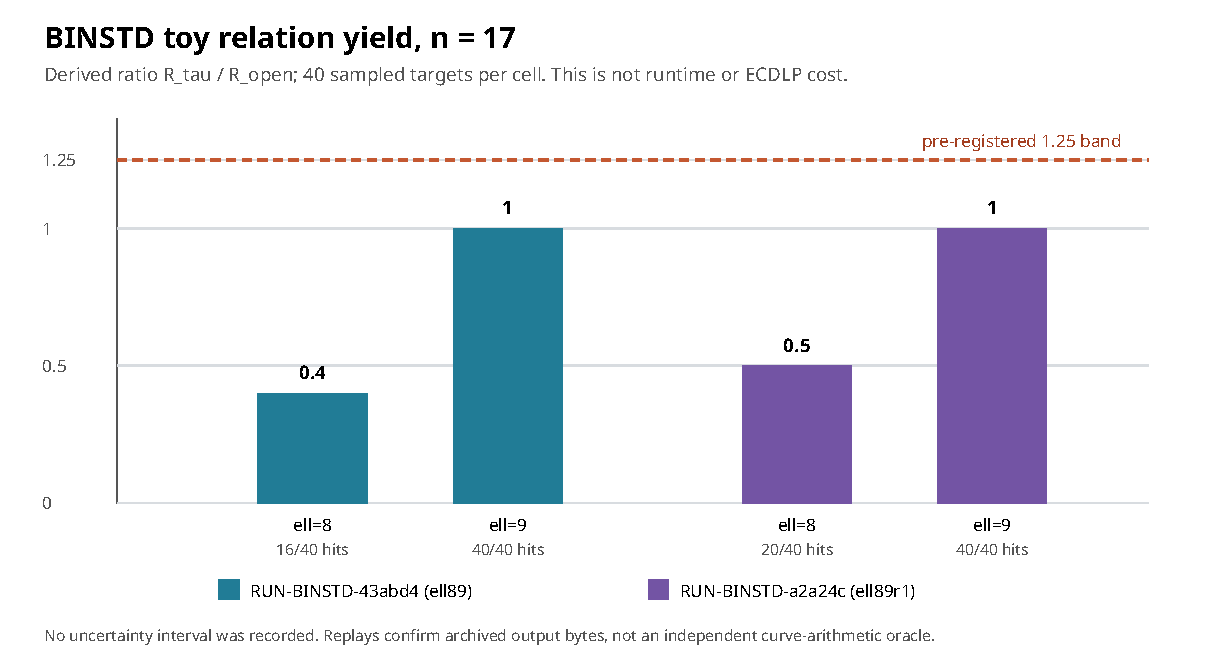
\includegraphics[width=0.98\linewidth]{yield-ratios.pdf}
\end{center}

Both freshly generated yield matrices, admissible-dimension files, and
results notes match the archived bytes exactly. Raw-result payloads match
after excluding the new timestamps. The source files, dated specifications,
and Stage-0 freeze artifacts match their recorded SHA-256 pins. The committed
\texttt{receipt.json} lists all hashes; a second end-to-end invocation of the
committed replay command reproduced it byte for byte. The first local replays took 355.8 and
315.6 seconds on Python 3.9.25; these are not benchmark timings.
A one-count mutation in a copied matrix caused the verifier to fail before
writing a receipt, including under \texttt{python3 -O}.

\textbf{Scope.} The four recorded toy ratios lie below the pre-registered
1.25 band at $n=17$, $\ell\in\{8,9\}$, under the exhaustive $m=3$ pin.
The open arm hit all 40 targets in each cell, so its observed rate was 1;
the tau rate cannot exceed 1, making the 1.25 ratio unattainable on those
measured cells. This is a ceiling limit on the tested protocol.
An independent polynomial irreducibility calculation passed, and the
degree-1 and two degree-8 factors of $x^{17}-1$ multiplied out, giving
subset sums $\{0,1,8,9,16,17\}$. The normal-basis link to invariant
subspaces has no Lean proof here. A separate binary-field implementation
checked all $8^3$ ordered triple sums and the pair-membership shortcut on
12 constructed hits and 12 sampled misses per pinned runner. This bounded
control does not independently recompute the full panel or prove the runner
in Lean. No ECDLP
break, asymptotic transfer, runtime advantage, or rho comparison follows.
No uncertainty interval was recorded for the 40-target hit rates.

\textbf{Reproduce.} Run \texttt{python3 docs/reports/2026-10-22-binstd-ell89-replay/replay.py --run}
from the repository root. The detailed report and graph source are beside
this PDF. The canonical performance graphs were checked; the replay creates
no new speedup or attack-cost row.
\end{document}
